\documentclass{article}\usepackage[]{graphicx}\usepackage[]{color}
%% maxwidth is the original width if it is less than linewidth
%% otherwise use linewidth (to make sure the graphics do not exceed the margin)

\makeatletter
\def\maxwidth{ %
  \ifdim\Gin@nat@width>\linewidth
    \linewidth
  \else
    \Gin@nat@width
  \fi
}
\makeatother

\usepackage{framed}
\makeatletter

\definecolor{fgcolor}{rgb}{0.345, 0.345, 0.345}
\newcommand{\hlnum}[1]{\textcolor[rgb]{0.686,0.059,0.569}{#1}}%
\newcommand{\hlstr}[1]{\textcolor[rgb]{0.192,0.494,0.8}{#1}}%
\newcommand{\hlcom}[1]{\textcolor[rgb]{0.678,0.584,0.686}{\textit{#1}}}%
\newcommand{\hlopt}[1]{\textcolor[rgb]{0,0,0}{#1}}%
\newcommand{\hlstd}[1]{\textcolor[rgb]{0.345,0.345,0.345}{#1}}%
\newcommand{\hlkwa}[1]{\textcolor[rgb]{0.161,0.373,0.58}{\textbf{#1}}}%
\newcommand{\hlkwb}[1]{\textcolor[rgb]{0.69,0.353,0.396}{#1}}%
\newcommand{\hlkwc}[1]{\textcolor[rgb]{0.333,0.667,0.333}{#1}}%
\newcommand{\hlkwd}[1]{\textcolor[rgb]{0.737,0.353,0.396}{\textbf{#1}}}%



\usepackage{framed}
\makeatletter
\newenvironment{kframe}{%
 \def\at@end@of@kframe{}%
 \ifinner\ifhmode%
  \def\at@end@of@kframe{\end{minipage}}%
  \begin{minipage}{\columnwidth}%
 \fi\fi%
 \def\FrameCommand##1{\hskip\@totalleftmargin \hskip-\fboxsep
 \colorbox{shadecolor}{##1}\hskip-\fboxsep
     % There is no \\@totalrightmargin, so:
     \hskip-\linewidth \hskip-\@totalleftmargin \hskip\columnwidth}%
 \MakeFramed {\advance\hsize-\width
   \@totalleftmargin\z@ \linewidth\hsize
   \@setminipage}}%
 {\par\unskip\endMakeFramed%
 \at@end@of@kframe}
\makeatother

\definecolor{shadecolor}{rgb}{.97, .97, .97}
\definecolor{messagecolor}{rgb}{0, 0, 0}
\definecolor{warningcolor}{rgb}{1, 0, 1}
\definecolor{errorcolor}{rgb}{1, 0, 0}
\newenvironment{knitrout}{}{} % an empty environment to be redefined in TeX

\usepackage{alltt}
\usepackage{fancyhdr}
\pagestyle{fancy}
\usepackage{float}
\setlength{\parskip}{\smallskipamount}
\setlength{\parindent}{0pt}
\usepackage{amsthm}
\usepackage{amsmath}
\usepackage{wrapfig}
\usepackage{graphicx}
\usepackage{float}
\usepackage[margin=1in]{geometry}
\IfFileExists{upquote.sty}{\usepackage{upquote}}{}

\newtheorem{corollary}{Corollary}[section]
\newtheorem{theorem}{Theorem}
\newtheorem{example}{Example}
\newtheorem{question}{Question}
\newtheorem{remark}{Remark}[section]
\newtheorem{conjecture}{Conjecture}
\newtheorem{proposition}{Proposition}[section]
\newtheorem{definition}{Definition}[section]


\begin{document}


\title{Lab 4-Binary Classifier\\
Stat 215A, Fall 2014}

\author{Xiang (Lisha) Li, Jonathan Fischer, Andrew Do, Hye Soo Choi}

\maketitle

\section{Introduction}
Blah blah...

\section{EDA}
\subsection{Densities of NDAI, SD and CORR}

The following three plots gives us a sense of what can be learned from NDAI, SD and CORR.  The densities are grouped by their expert labels, red is for 'no cloud', green are for 'unknown' and blue for 'cloud'. We can see that NDAI has reasonably good separation between cloud and no cloud, in all three pictures, which is confirmed in our later modeling sections by Gini importance measures found in the random forest model and it's importance as a variable in LDA/QDA and logit models. SD does not have such a good separation within the lower regions of the SD values, however it is still clear that pixels labelled as clouds are the only values with higher SD values.  We thus expect the two features in combination can help determine whether a pixel with high NDAI should be labelled as a cloud by using the SD feature.  Finally CORR values appear to be a good separator for image 2, but much less so for image 1.  This uneven distribution of CORR values between images prompted us to cross validate our models across images, in addition to the folds created by dividing each image into 4 quadrants. 

\begin{figure}[H]
\minipage{0.32\textwidth}
  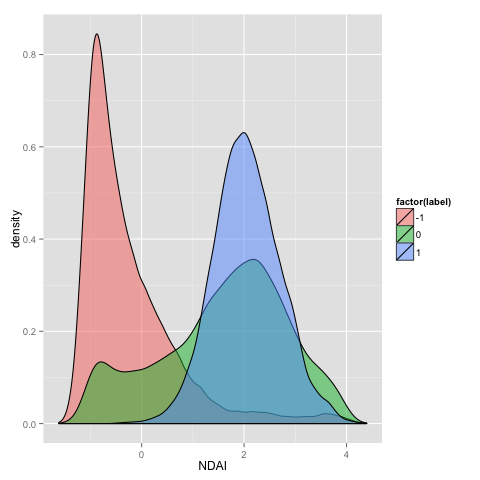
\includegraphics[width=\linewidth, height = 100pts ]{NDAI1.png}
\endminipage\hfill
\minipage{0.32\textwidth}
  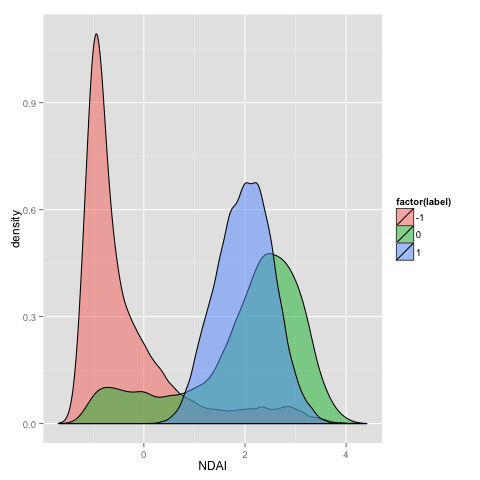
\includegraphics[width=\linewidth, height = 100pts]{NDAI2.png}
\endminipage\hfill
\minipage{0.32\textwidth}%
  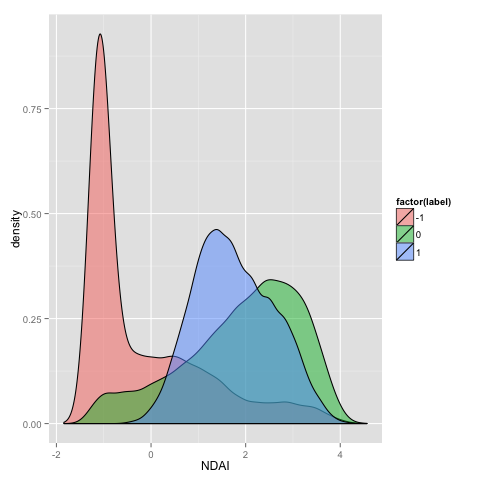
\includegraphics[width=\linewidth, height = 100pts]{NDAI3.png}
\endminipage
  \caption{NDAI density plot for Image 1, 2, 3 (respectively).}\label{}
\end{figure}

\begin{figure}[H]
\minipage{0.32\textwidth}
  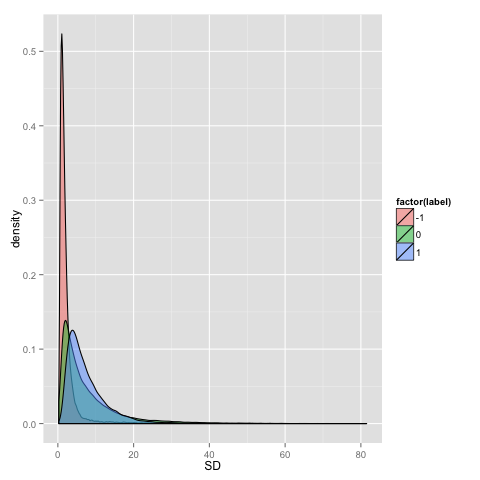
\includegraphics[width=\linewidth, height = 100pts]{SD1.png}
\endminipage\hfill
\minipage{0.32\textwidth}
  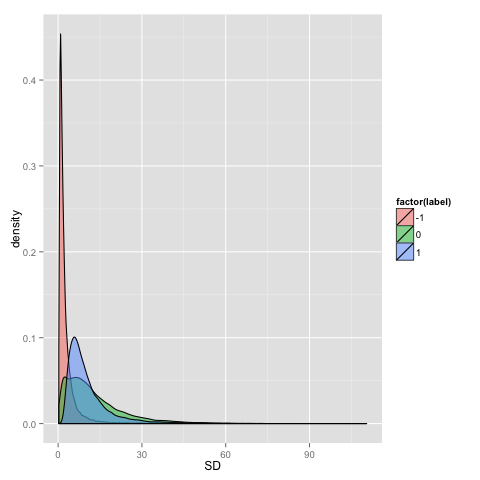
\includegraphics[width=\linewidth, height = 100pts]{SD2.png}
\endminipage\hfill
\minipage{0.32\textwidth}%
  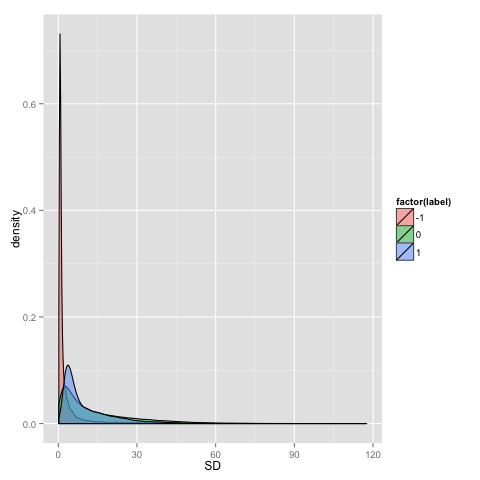
\includegraphics[width=\linewidth, height = 100pts]{SD3.png}
\endminipage
  \caption{SD density plot for Image 1, 2, 3 (respectively).}
\end{figure}

\begin{figure}[H]
\minipage{0.32\textwidth}
  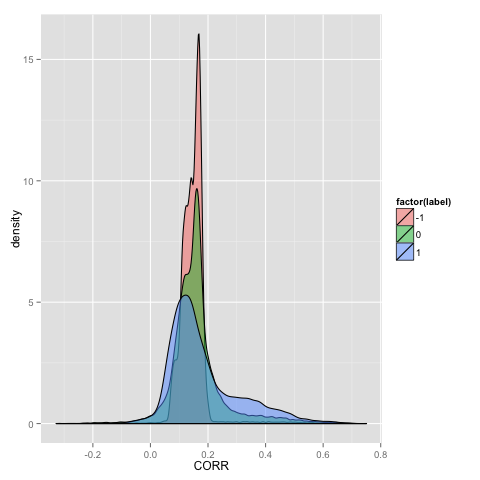
\includegraphics[width=\linewidth, height = 100pts]{CORR1.png}
\endminipage\hfill
\minipage{0.32\textwidth}
  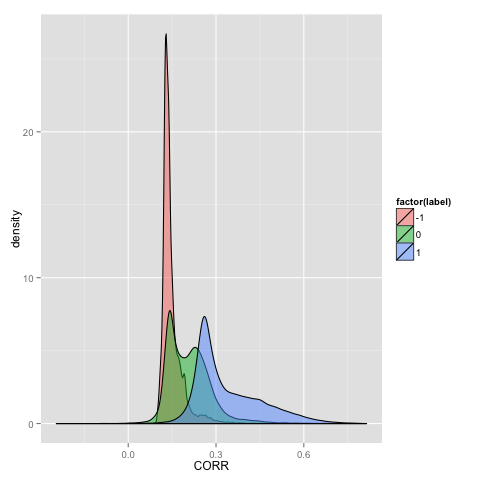
\includegraphics[width=\linewidth, height = 100pts]{CORR2.png}
\endminipage\hfill
\minipage{0.32\textwidth}%
  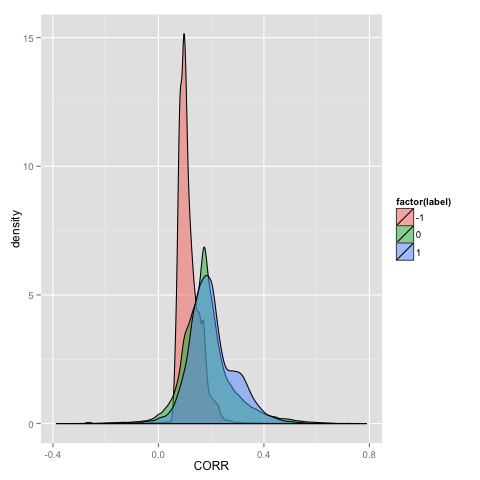
\includegraphics[width=\linewidth, height = 100pts]{CORR3.png}
\endminipage
  \caption{CORR density plot for Image 1, 2, 3 (respectively).}\label{}
\end{figure}


\begin{figure}[H]
\minipage{0.32\textwidth}
  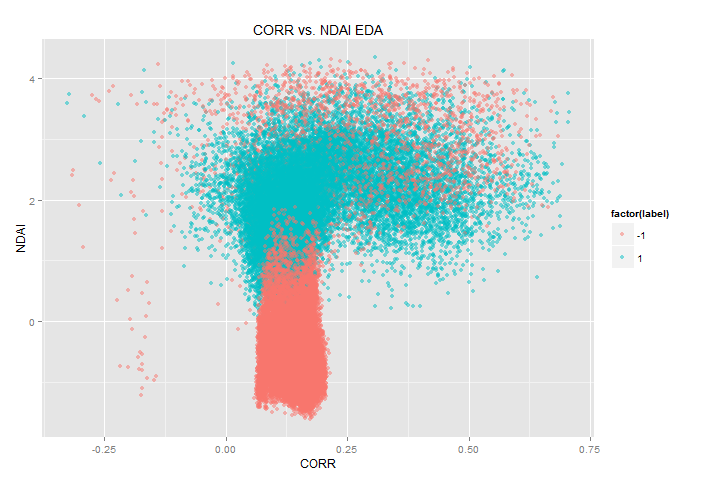
\includegraphics[width=\linewidth]{CORRvsNDAI.png}
  \caption{CORR vs. NDAI Plot of Image 1}\label{}
\endminipage\hfill
\minipage{0.32\textwidth}
  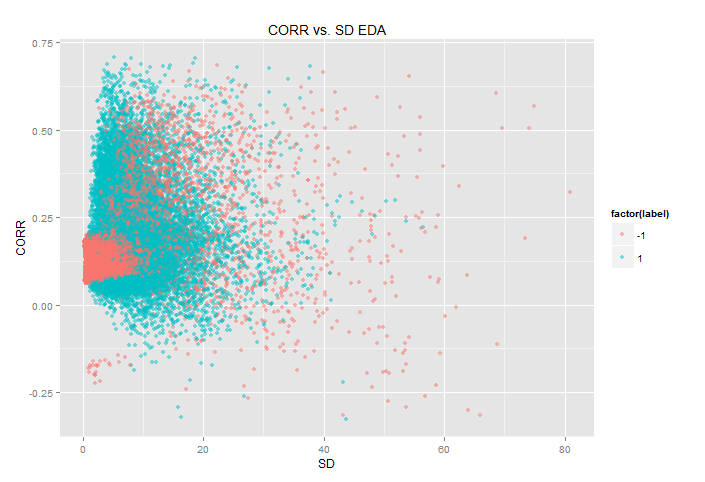
\includegraphics[width=\linewidth]{CORRvsSD.png}
  \caption{CORR vs. SD Plot of Image 1}\label{}
\endminipage\hfill
\minipage{0.32\textwidth}%
  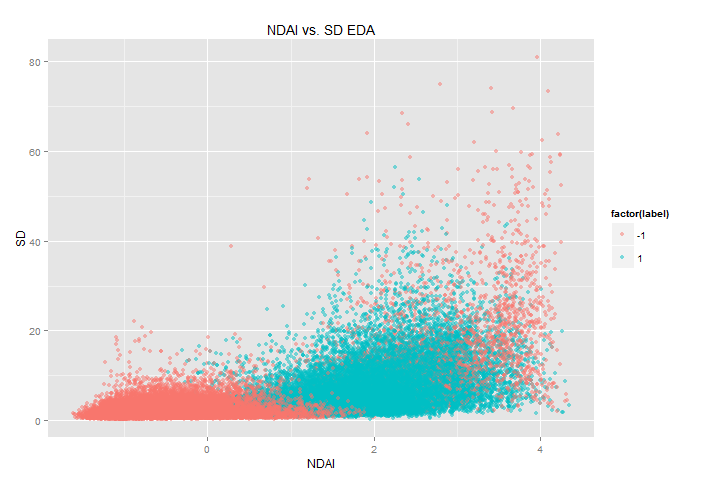
\includegraphics[width=\linewidth]{NDAIvsSD.png}
  \caption{NDAI vs. SD Plot of Image1}\label{}
\endminipage
\end{figure}

\begin{figure}[H]
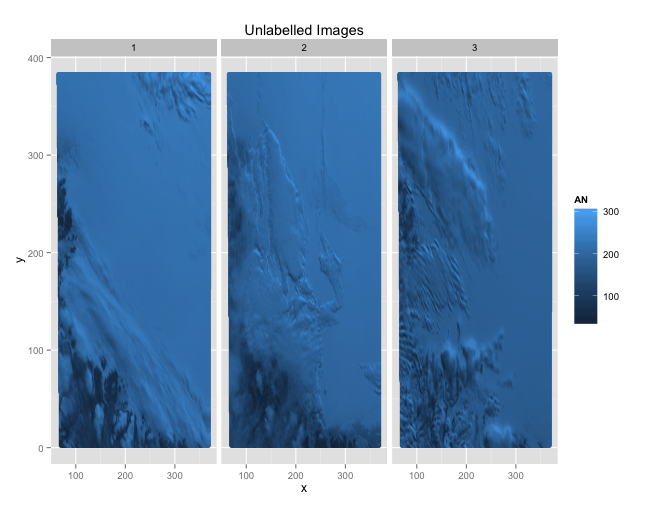
\includegraphics[width = 18cm, height=8cm]{RAWEDA.png}
\caption{Raw images with AN radiances.}
\end{figure}

\begin{figure}[H]
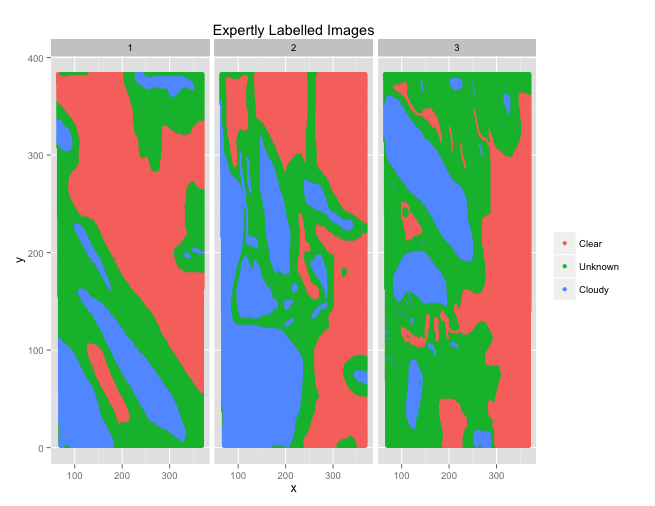
\includegraphics[width = 18cm, height=8cm]{EXPERTSEDA.png}
\caption{Images with expert classifications.}
\end{figure}

\begin{figure}[H]
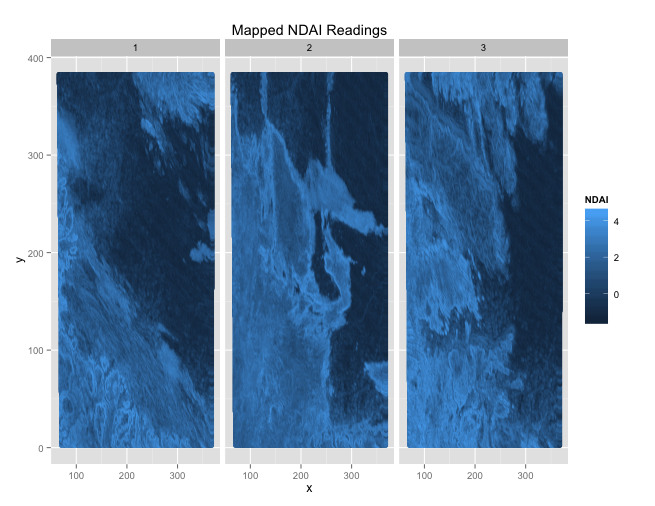
\includegraphics[width = 18cm, height = 8cm]{NDAIEDA.png}
\caption{Mapped NDAI readings. We see good correspondence between larger values and presence of clouds.}
\end{figure}

\begin{figure}[H]
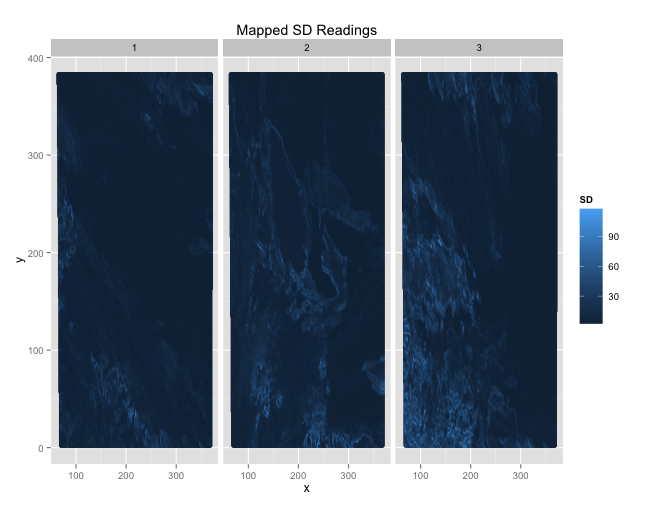
\includegraphics[width = 18cm, height = 8cm]{SDEDA.png}
\caption{Mapped SD readings. Higher values show cloud boundaries, though also shows uneven terrain.}
\end{figure}

\begin{figure}[H]
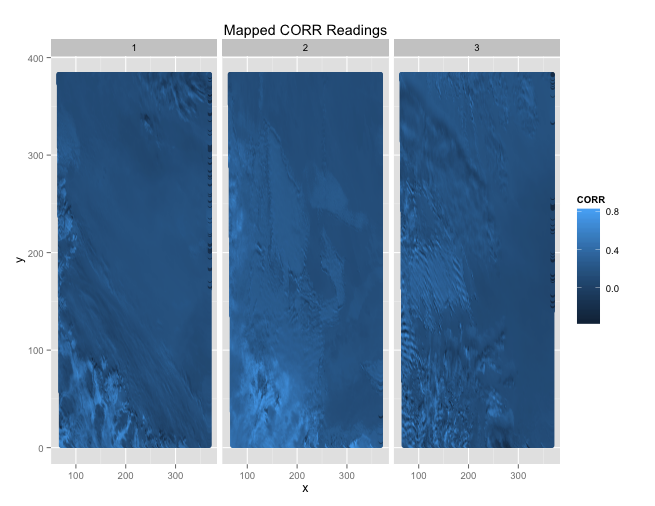
\includegraphics[width = 18cm, height = 8cm]{CORREDA.png}
\caption{Mapped CORR readings. Cloudy regions tend to be lighter, but not as strongly as in NDAI.}
\end{figure}

\section{Modeling}

\subsection{LDA}

\subsection{QDA}

\begin{figure}[h]
\minipage{0.49\textwidth}
  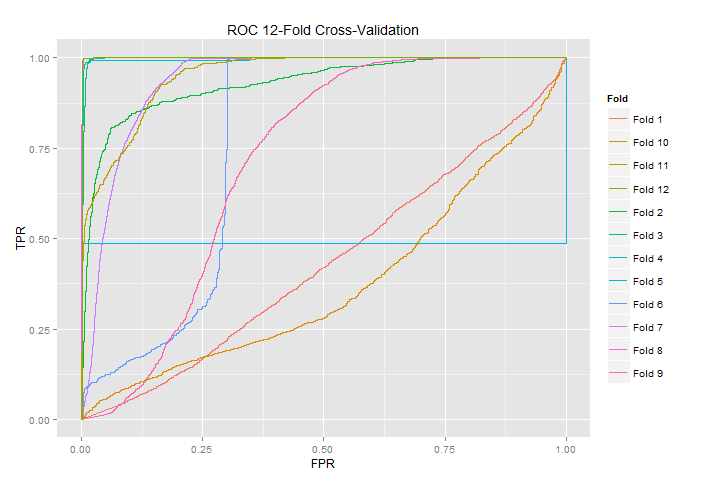
\includegraphics[width=\linewidth]{QDArocCV.png}
  \caption{Response Operator Curve for 12-fold Cross-valudation of QDA}\label{}
\endminipage\hfill
\minipage{0.49\textwidth}
  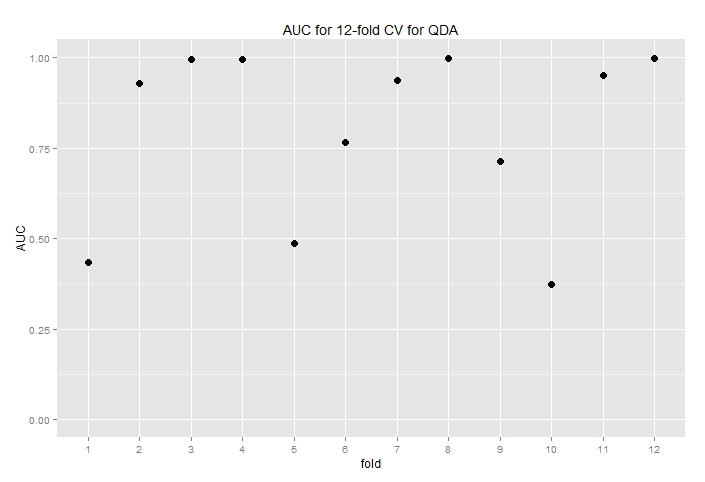
\includegraphics[width=\linewidth]{AUCcvQDA.png}
  \caption{AUC for QDA Classifiers}\label{rocauc}
\endminipage\hfill
\end{figure}

Cross-validation for QDA revealed that while the method works extremely well in some cases, producing AUC scores of almost 1, it sometimes fails to perform better than even the theoretical random classifier.  In particular, the classifier does not seem to be good at discerning snow from clouds in regions where there are many dark pixels.  For example, during cross-validation, the watery bottom-left quadrant of image 2 and ridge-ridden left edge of image 3 poses significant problems to our classifiers.

\subsection{Logit/Probit}
The logit model obtained via averaging after 12-fold cross-validation has $y_i = -3.356 + 1.900 * NDAI_i - 0.074 * SD_i + 9.002 * CORR_i$ where $P_i$(Cloud) = $ \frac{1}{1 + e^{-y_i}}$. 

\begin{figure}[H]
\begin{center}
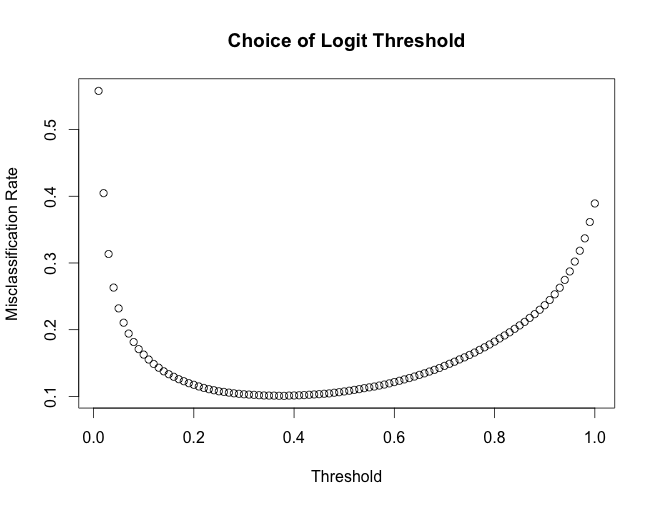
\includegraphics[scale = .35]{threshold.png}
\caption{We see a minimum in misclassification rate at .38.}
\end{center}
\end{figure}

\begin{figure}[H]
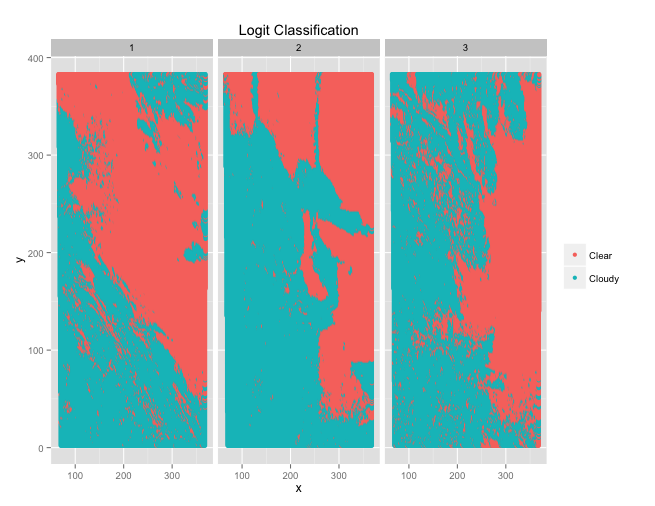
\includegraphics[width = 18cm, height = 8cm]{LogitClassification.png}
\caption{Binary classifications with threshold = .38 for logit trained via 12-fold CV.}
\end{figure}

\begin{figure}[H]
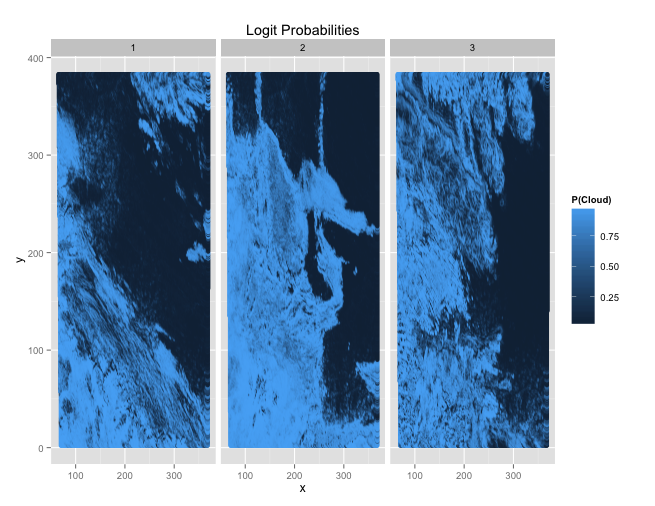
\includegraphics[width = 18cm, height = 8cm]{LogitProbabilities.png}
\caption{Probabilities for logit trained via 12-fold CV.}
\end{figure}

\begin{figure}[H]
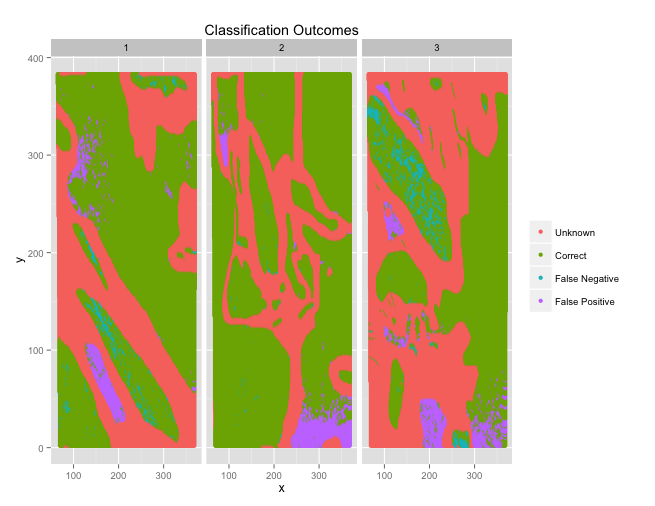
\includegraphics[width = 18cm, height = 10cm]{ClassificationOutcomes.png}
\caption{Classification results from logit with respect to the expert labels.}
\end{figure}

\begin{figure}[H]
\begin{center}
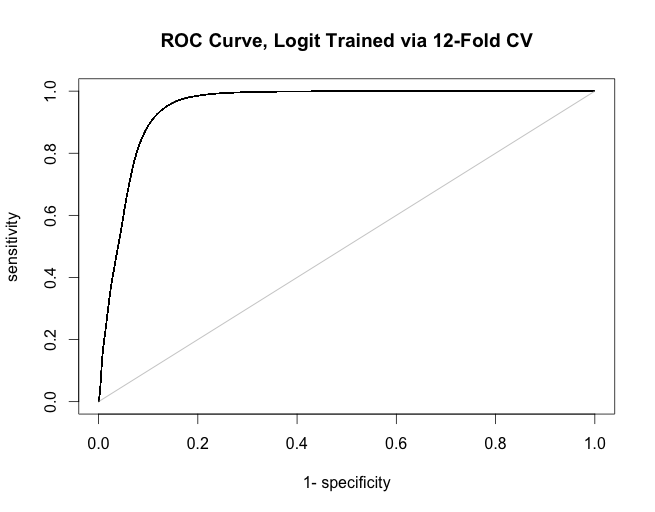
\includegraphics[scale = .5]{LogitROC.png}
\caption{ROC curve for our Logit model. AUC is .95.}
\end{center}
\end{figure}

\begin{figure}[H]
\begin{center}
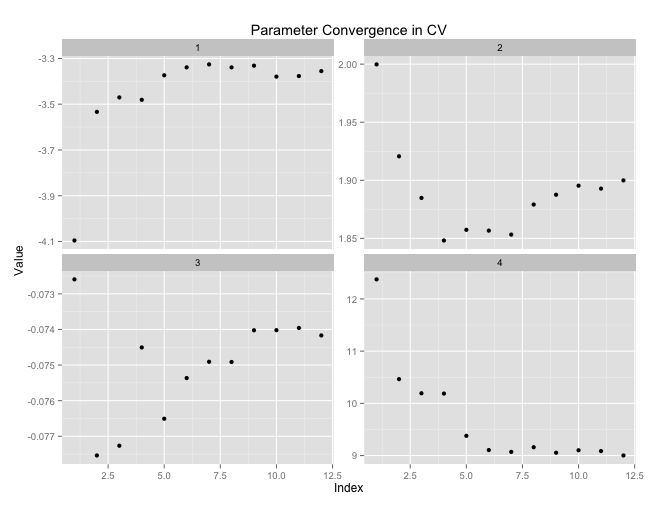
\includegraphics[scale = .5]{ParameterConvergence.png}
\caption{Coefficient values through iterations of 12-fold CV.}
\end{center}
\end{figure}

\subsection{Random Forest}

For random forest, as in all the other classifiers, we divided the three images into equal sized quadrants (2X2) rectangles in order to do 12 fold validation on the dataset.  That is, for each iteration of the validation, we dropped one of the quadrants as a test set, and trained on the remaining 11 quadrants.  Keeping the images segments disjoint and continuous ensured that our models were picking up on `higher' level structure of the dataset, and not the continuous variation of neighbouring pixels.  We also trained on each image and tested on the remaining two.  To test convergence, one of the things we did was increase the training set from including 1 quadrant, to including 2 quadrants, up to including 11 quadrants (using the complement as the test set).  For each of the 3 aforementioned classes of training, we trained on a range of forest sizes, from 2 trees to 50.     Here are the results: 

Finally, this entire set of training models was done with all the features, and then restricted to only SD, CORR and NDAI.  These three were particularly chosen because their GiniImportance was consistently ranked at least 2fold above the next highest in all the cross validations. As we also saw with the random forest model that just used SD, CORR, NDAI, it did not fare poorly compared to training the forests on all 9 predictors.  

\begin{figure}[h]
\minipage{0.32\textwidth}
  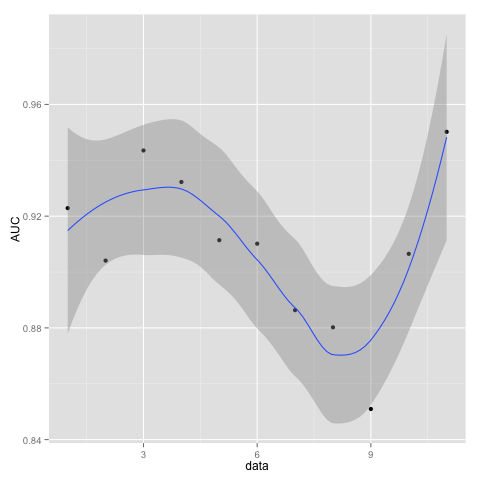
\includegraphics[width=\linewidth]{AUCconverge.png}
  \caption{Smoothed convergence of AUC for growing training set 50 trees and 3 features}\label{}
\endminipage\hfill
\minipage{0.32\textwidth}
  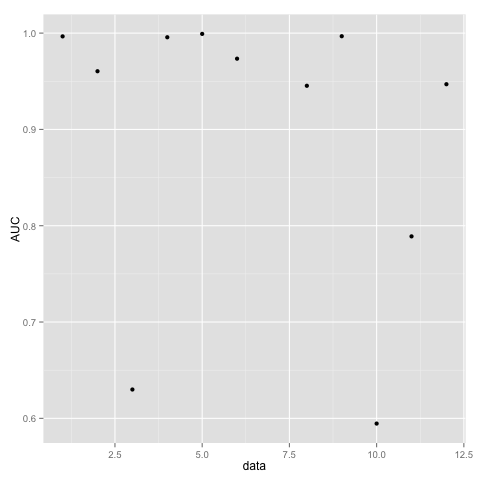
\includegraphics[width=\linewidth]{CVAUC.png}
  \caption{AUC of test set in each fold with 50 trees and 3 features}\label{}
\endminipage\hfill
\minipage{0.32\textwidth}%
  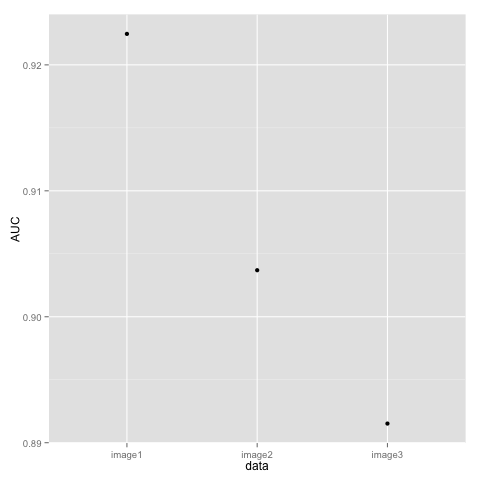
\includegraphics[width=\linewidth]{imageAUC.png}
  \caption{AUC of the three images with 50 trees and 3 features}\label{}
\endminipage
\end{figure}


{\bf Cross Validation ROC curves}

\begin{figure}[h]
\minipage{0.32\textwidth}
  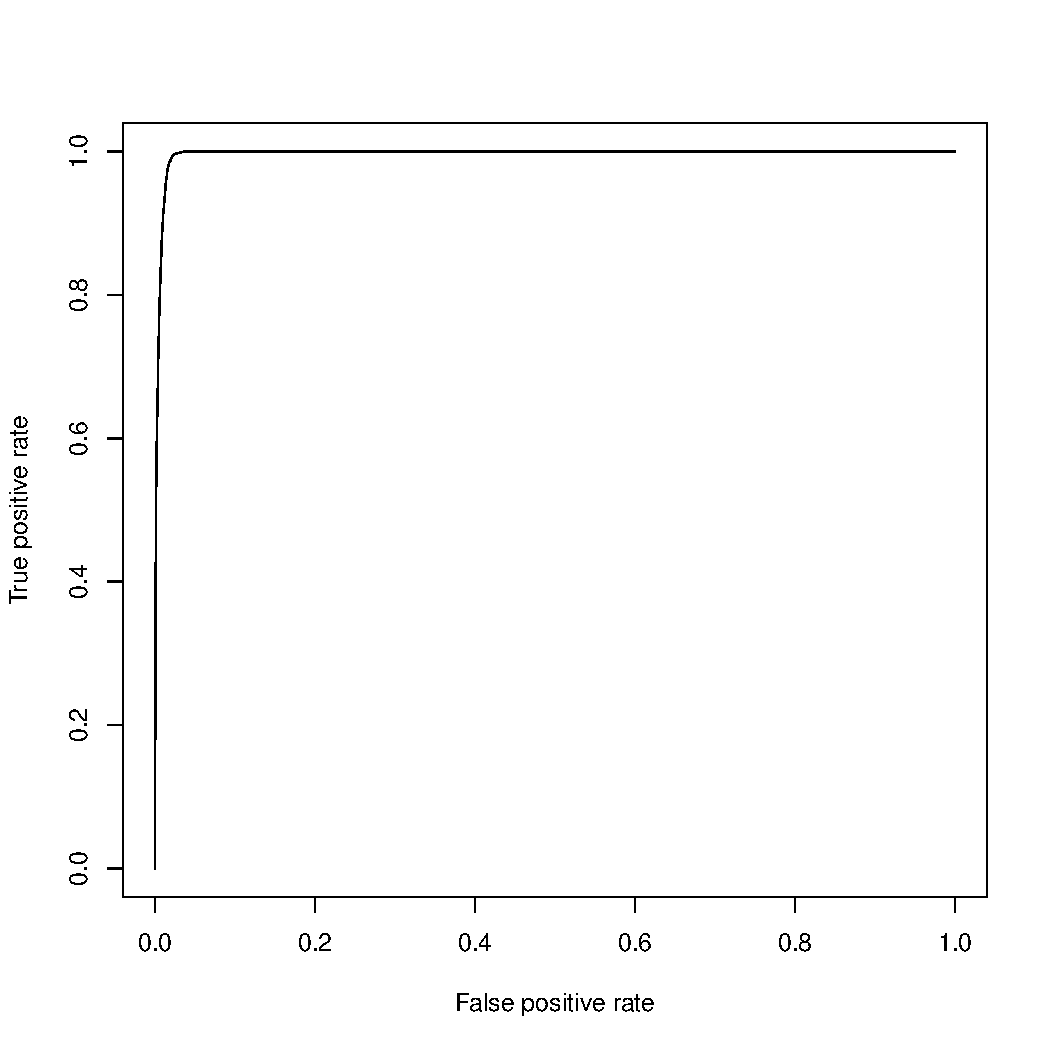
\includegraphics[width=\linewidth]{ROC_block1.pdf}
  \caption{ROC fold 1}\label{}
\endminipage\hfill
\minipage{0.32\textwidth}
  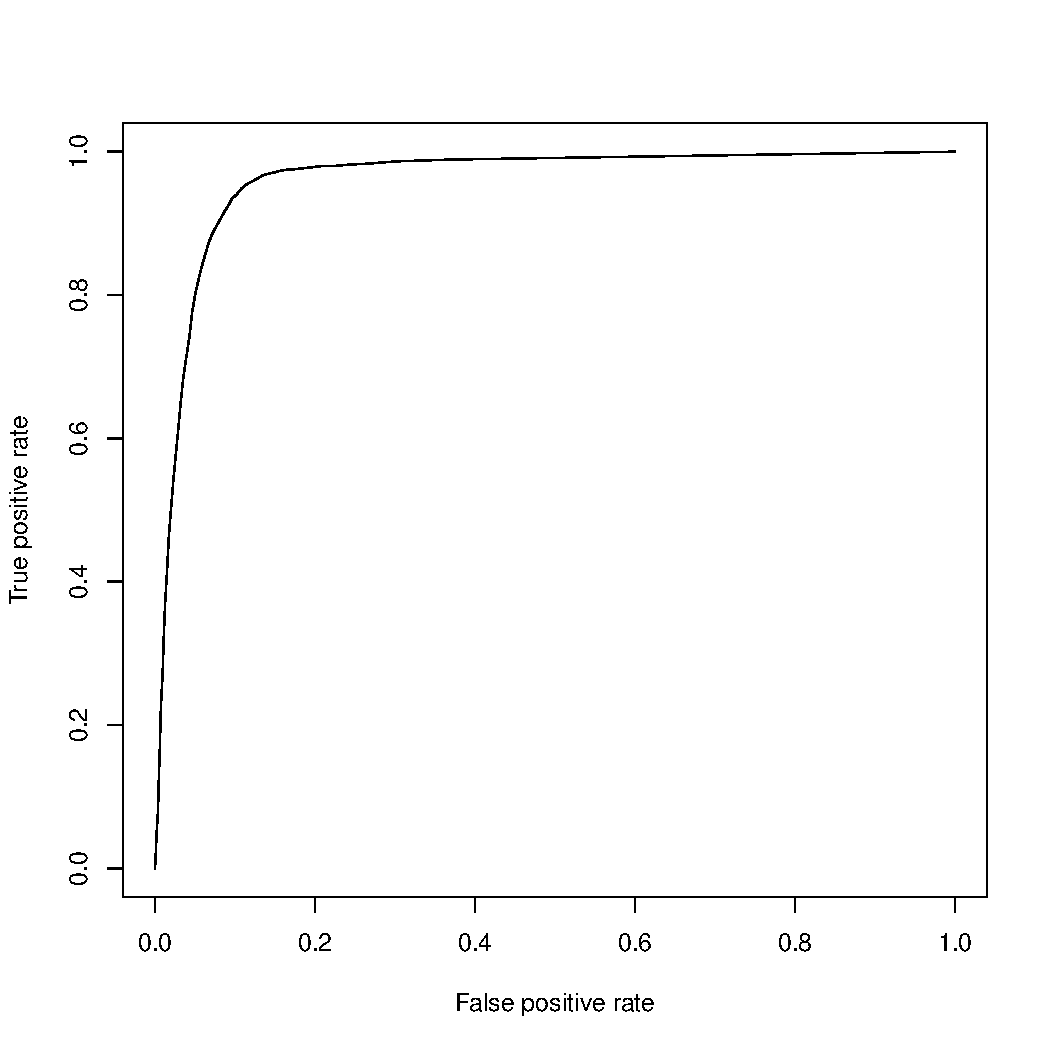
\includegraphics[width=\linewidth]{ROC_block2.pdf}
  \caption{ROC fold 2}\label{}
\endminipage\hfill
\minipage{0.32\textwidth}%
  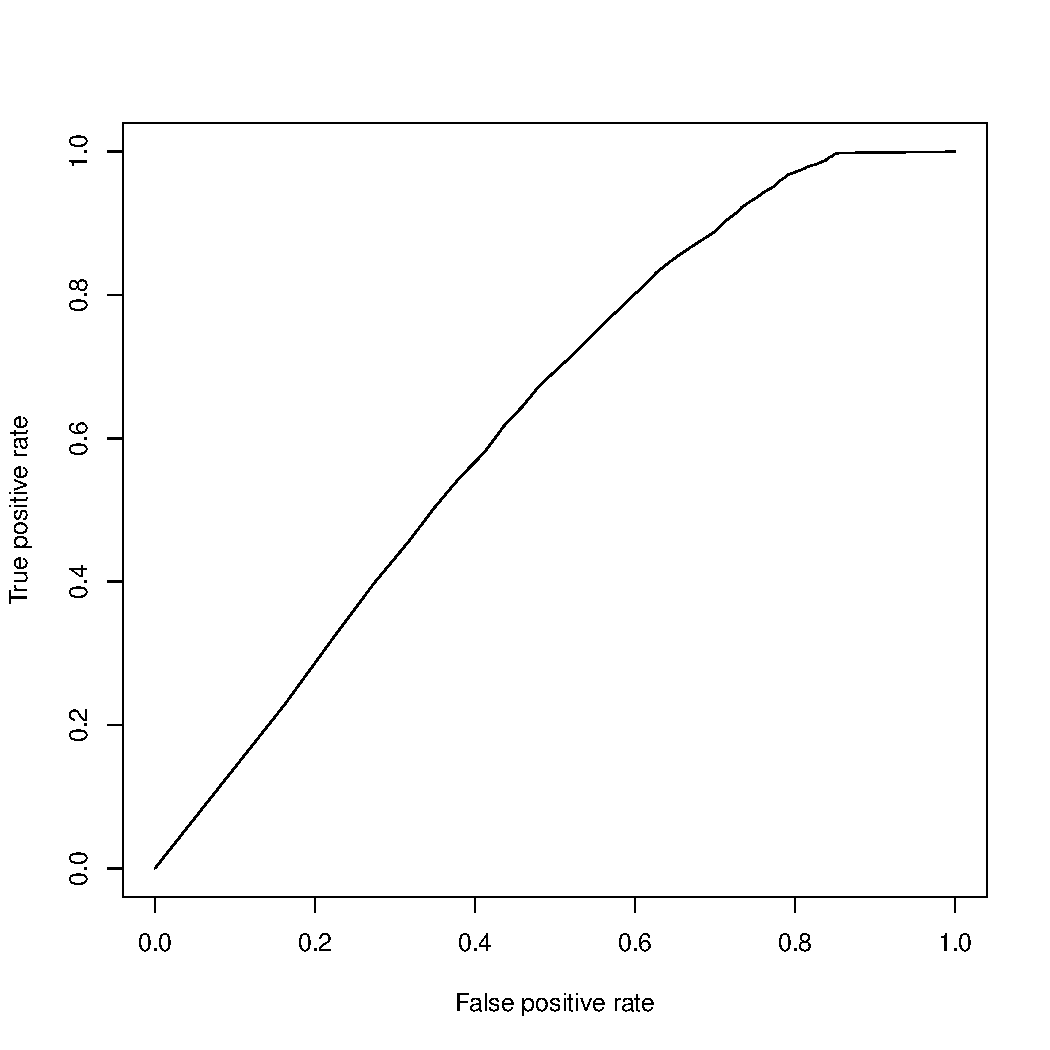
\includegraphics[width=\linewidth]{ROC_block3.pdf}
  \caption{ROC fold 3}\label{}
\endminipage
\end{figure}

\begin{figure}[h]
\minipage{0.32\textwidth}
  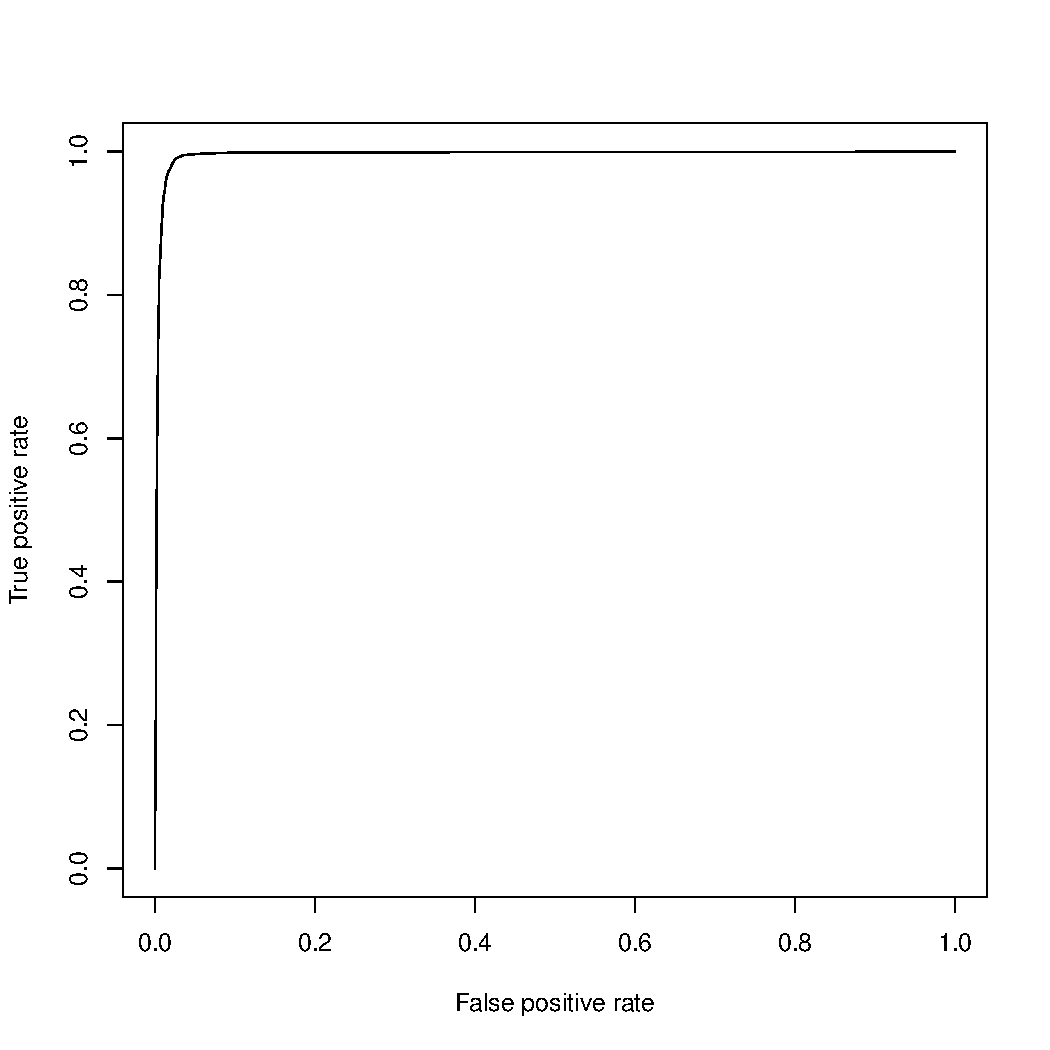
\includegraphics[width=\linewidth]{ROC_block4.pdf}
  \caption{ROC fold 4}\label{}
\endminipage\hfill
\minipage{0.32\textwidth}
  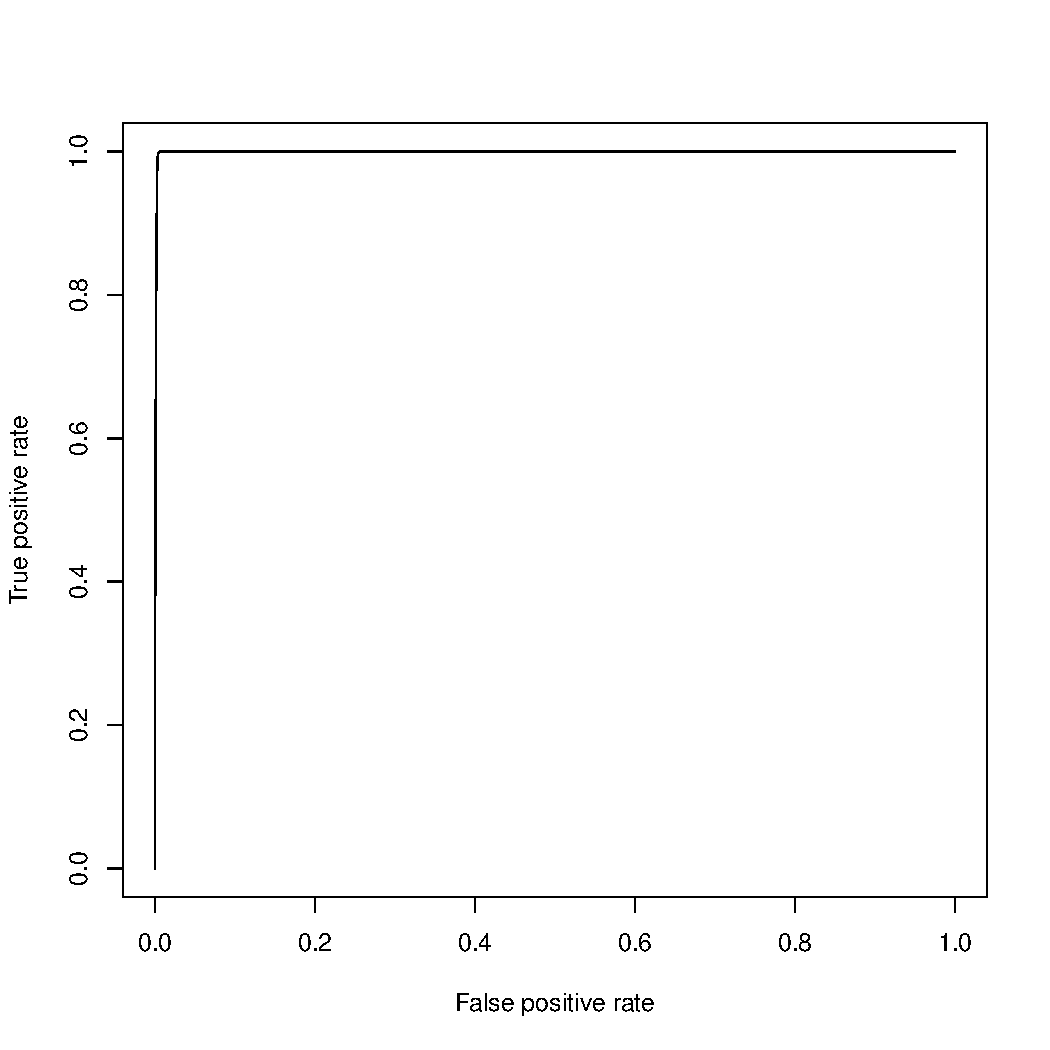
\includegraphics[width=\linewidth]{ROC_block5.pdf}
  \caption{ROC fold 5}\label{}
\endminipage\hfill
\minipage{0.32\textwidth}%
  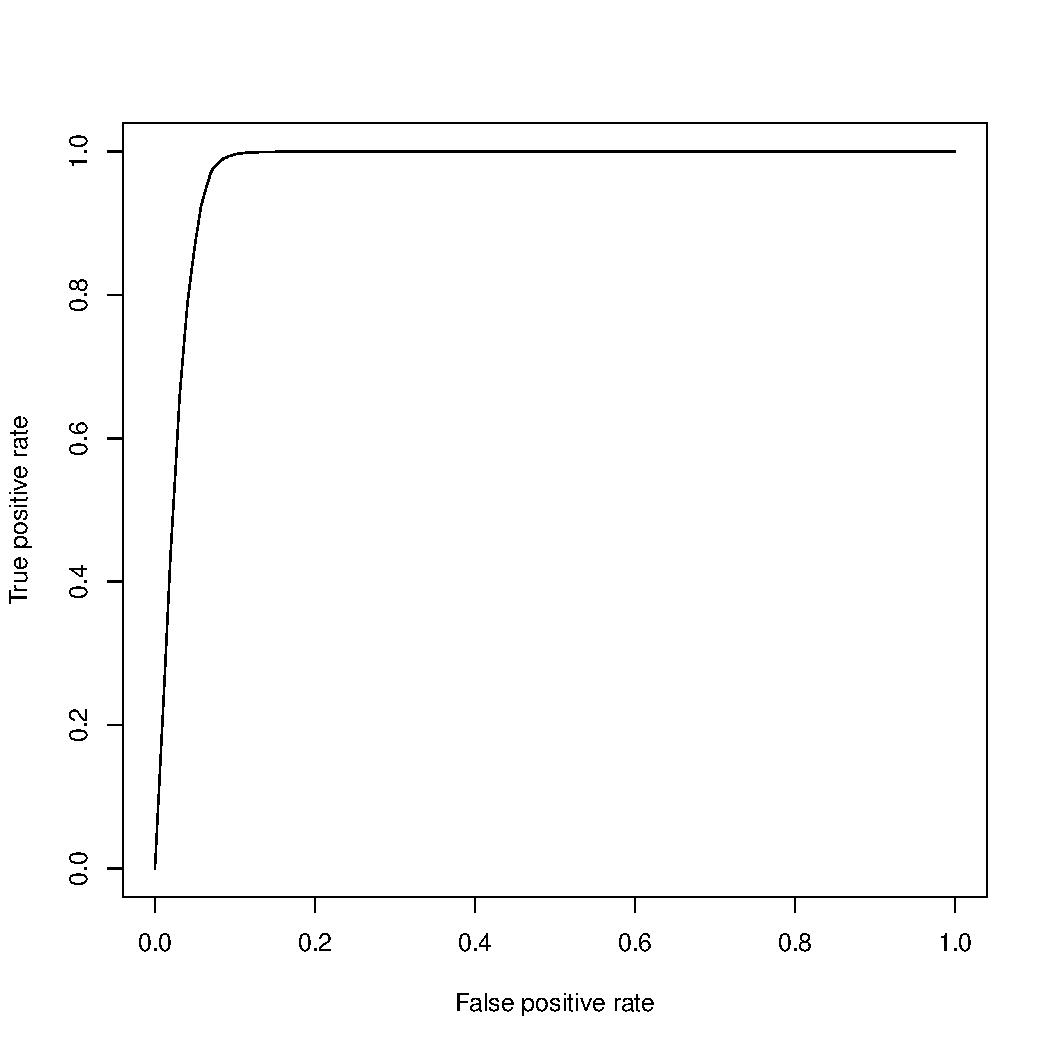
\includegraphics[width=\linewidth]{ROC_block6.pdf}
  \caption{ROC fold 6}\label{}
\endminipage
\end{figure}

\begin{figure}[h]
\minipage{0.32\textwidth}
  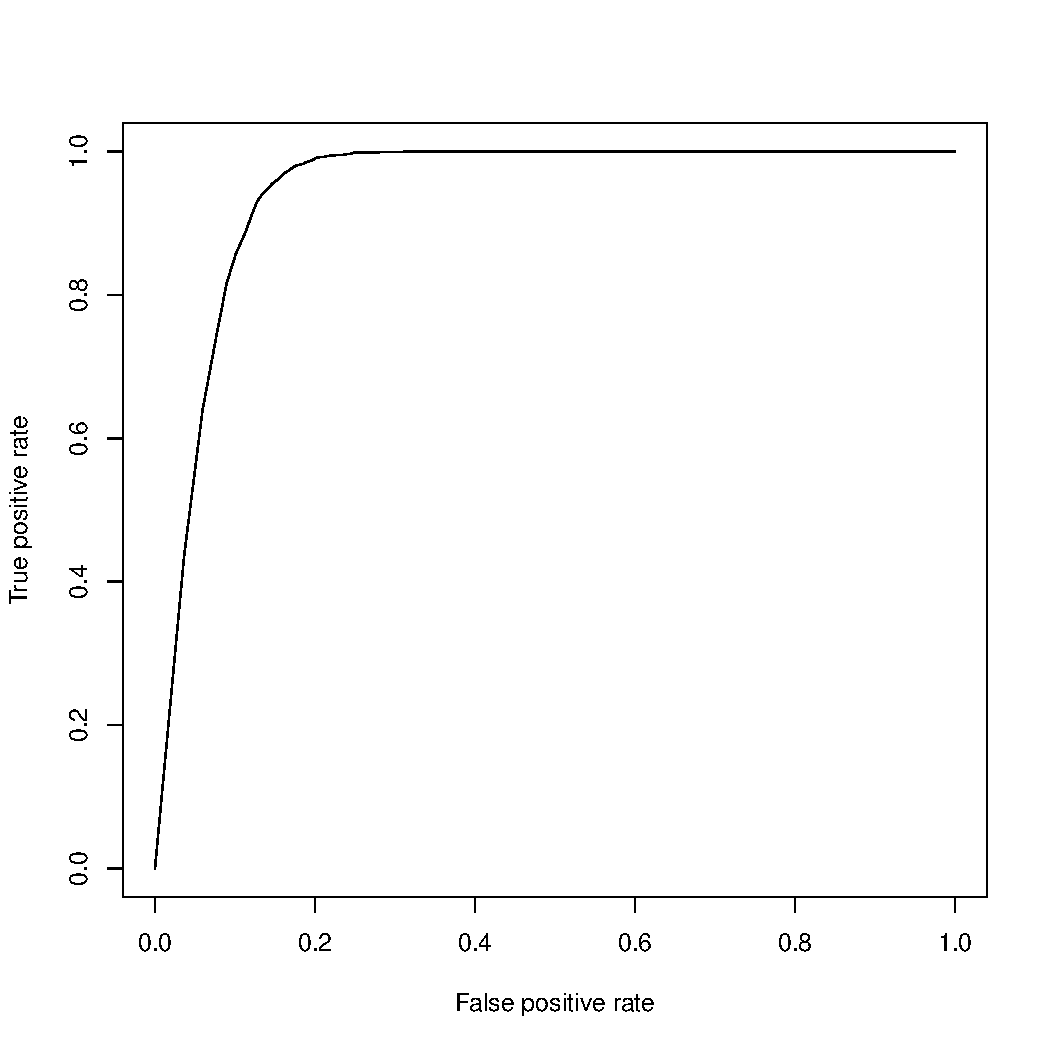
\includegraphics[width=\linewidth]{ROC_block8.pdf}
  \caption{ROC fold 8}\label{}
\endminipage\hfill
\minipage{0.32\textwidth}
  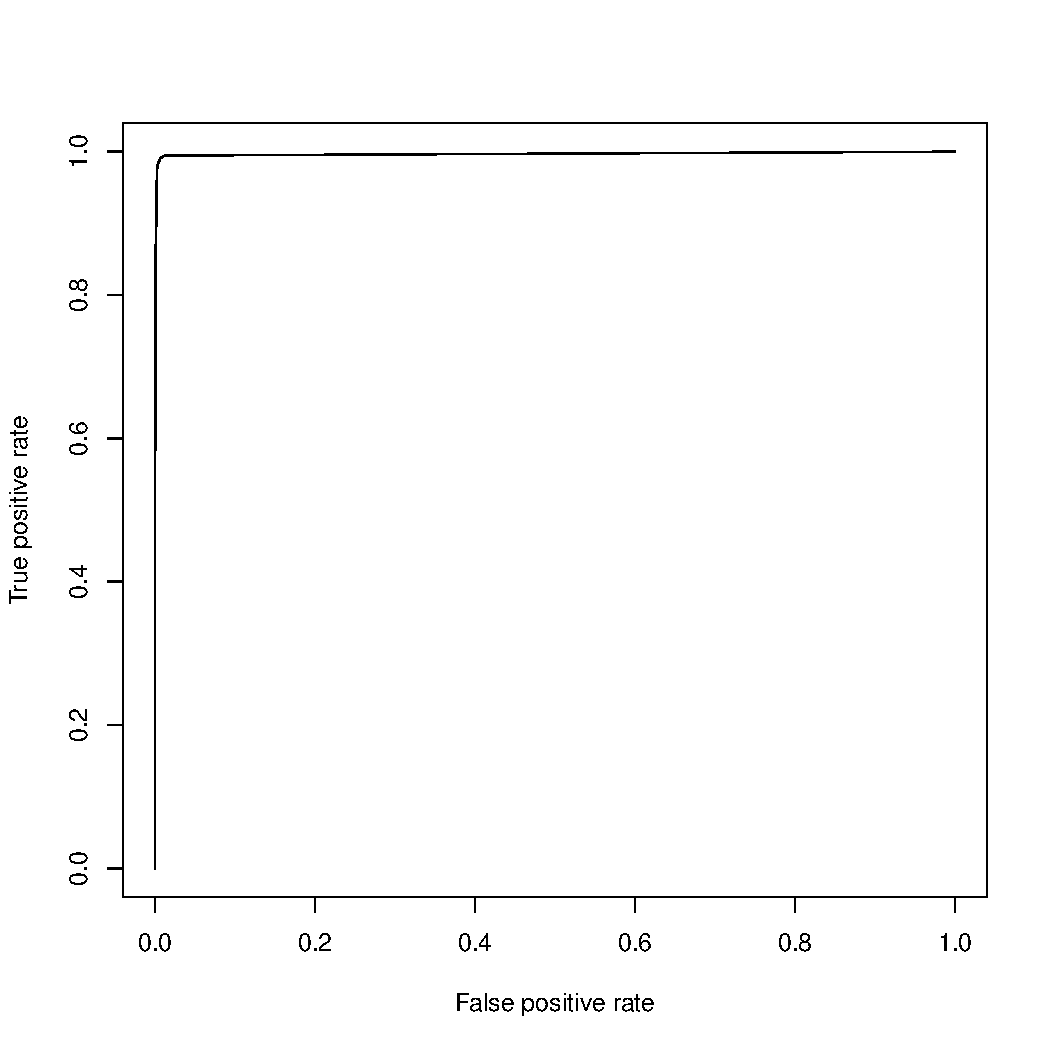
\includegraphics[width=\linewidth]{ROC_block9.pdf}
  \caption{ROC fold 9}\label{}
\endminipage\hfill
\minipage{0.32\textwidth}%
  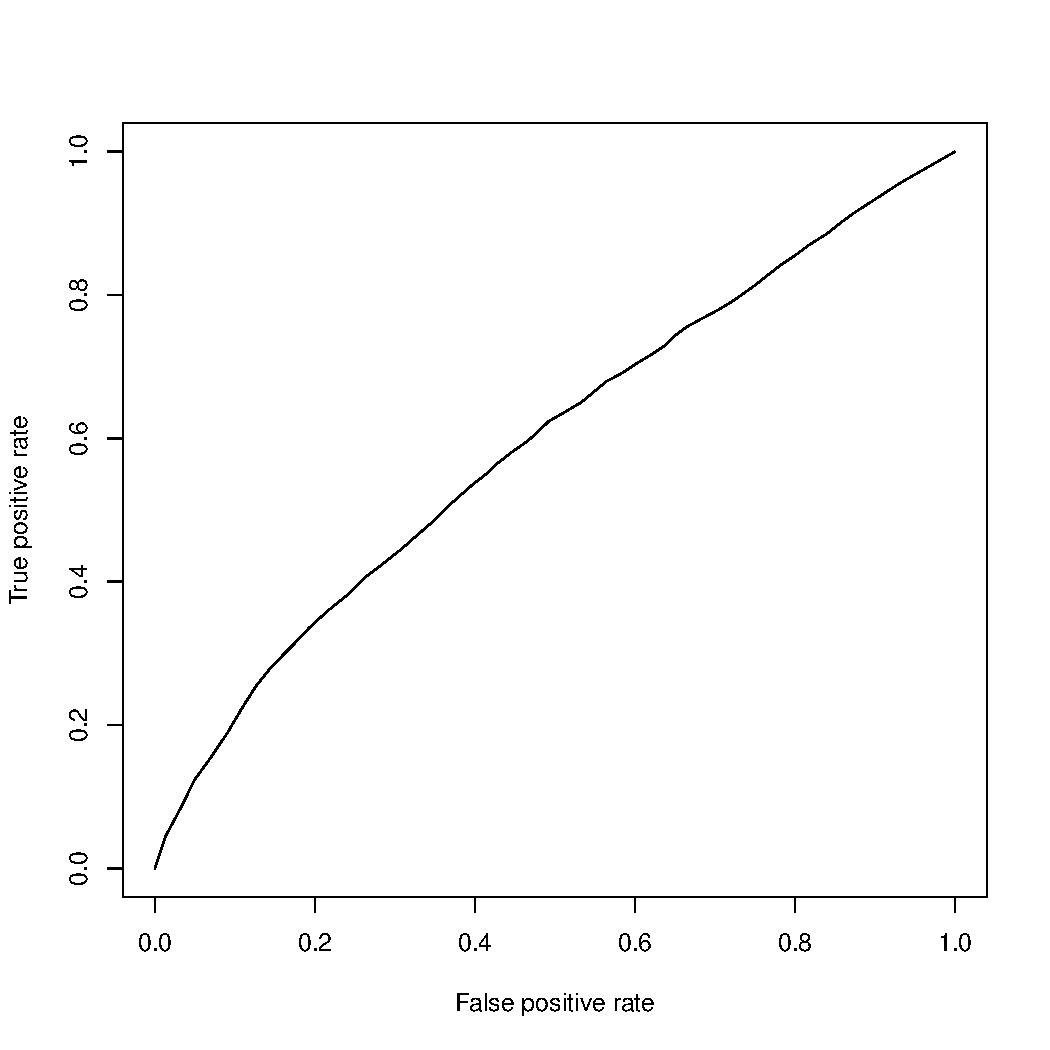
\includegraphics[width=\linewidth]{ROC_block10.pdf}
  \caption{ROC fold 10}\label{}
\endminipage
\end{figure}

\begin{figure}[h]
\minipage{0.32\textwidth}
  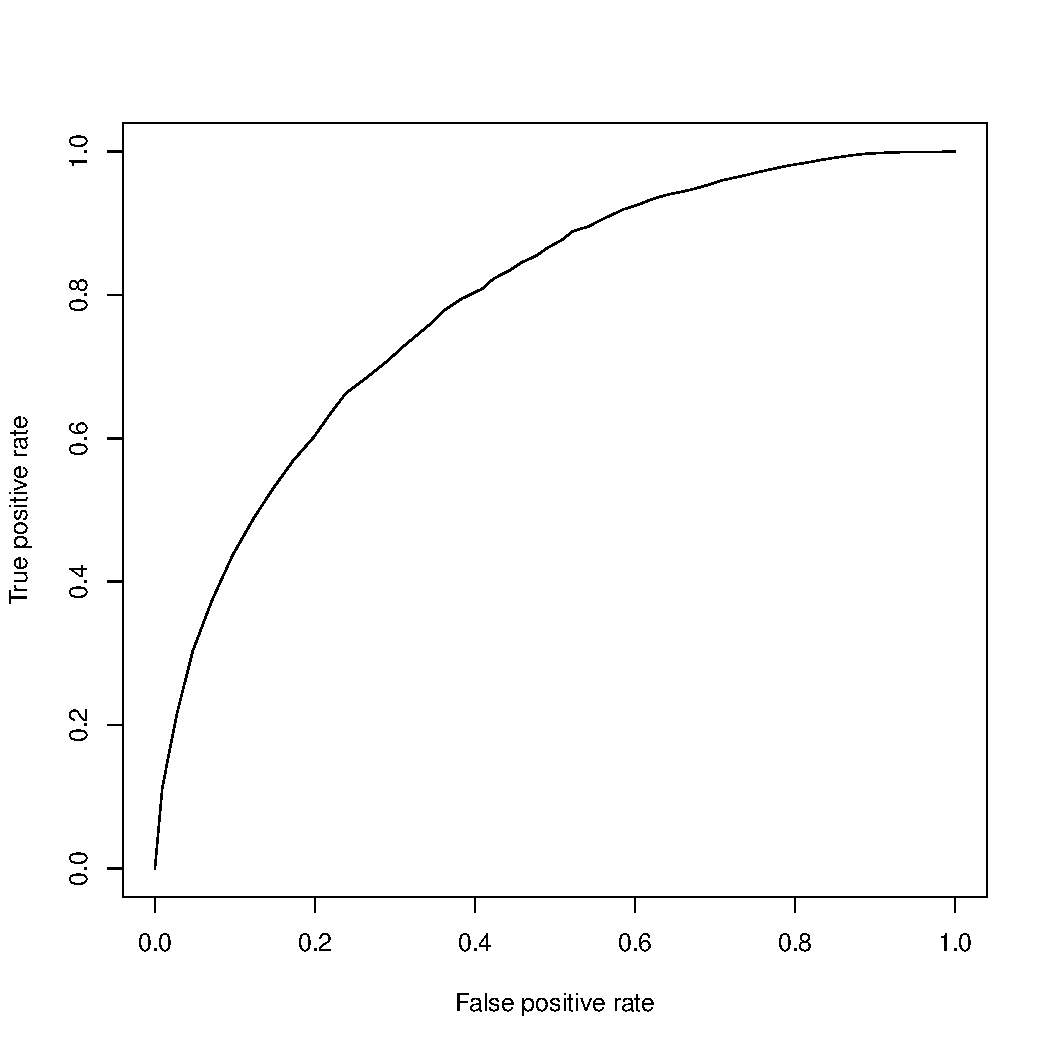
\includegraphics[width=\linewidth]{ROC_block11.pdf}
  \caption{ROC fold 11}\label{}
\endminipage\hfill
\minipage{0.32\textwidth}%
  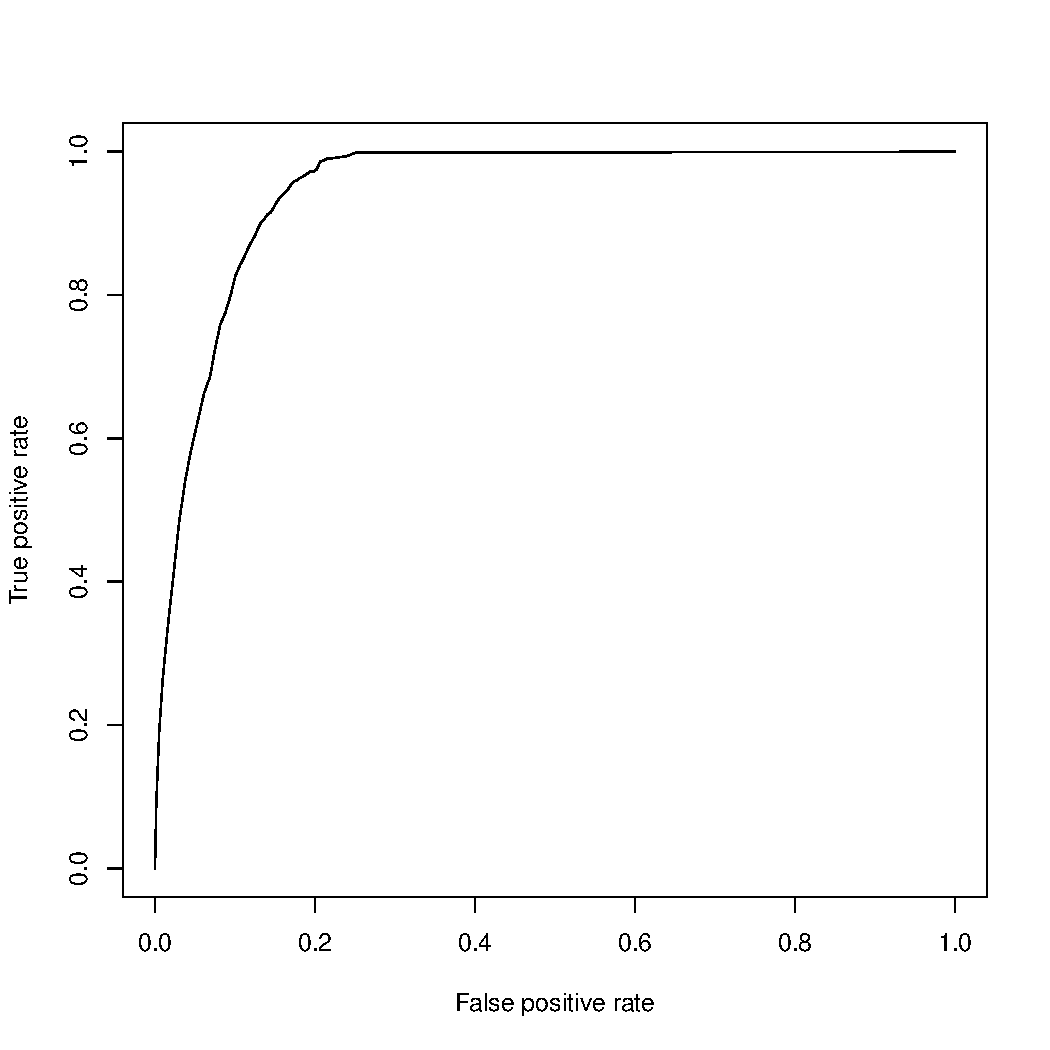
\includegraphics[width=\linewidth]{ROC_block12.pdf}
  \caption{ROC fold 12}\label{}
\endminipage
\end{figure}

{\bf ROC curves for cross validation between images} 

\begin{figure}[h]
\minipage{0.32\textwidth}
  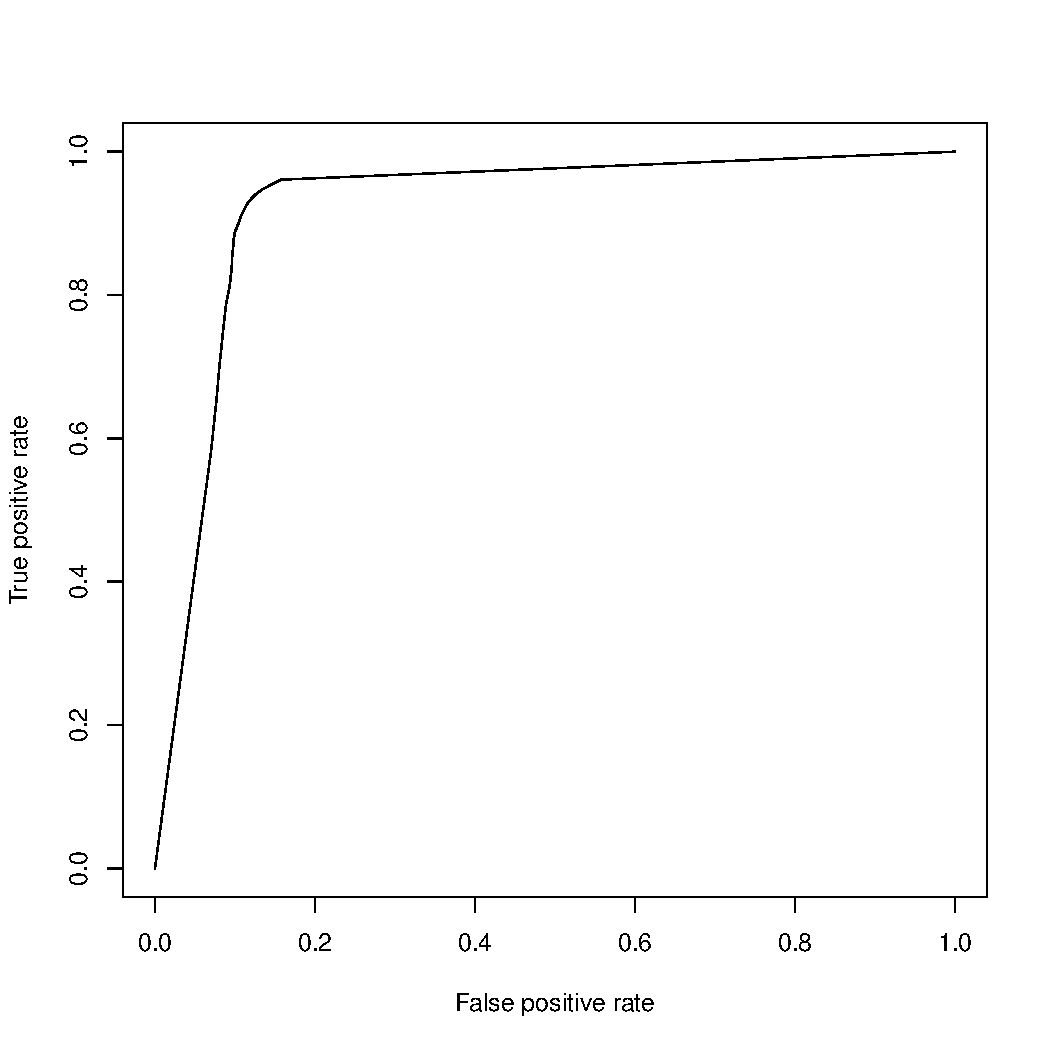
\includegraphics[width=\linewidth]{ROC_image1.pdf}
  \caption{Trained on image1}\label{}
\endminipage\hfill
\minipage{0.32\textwidth}
  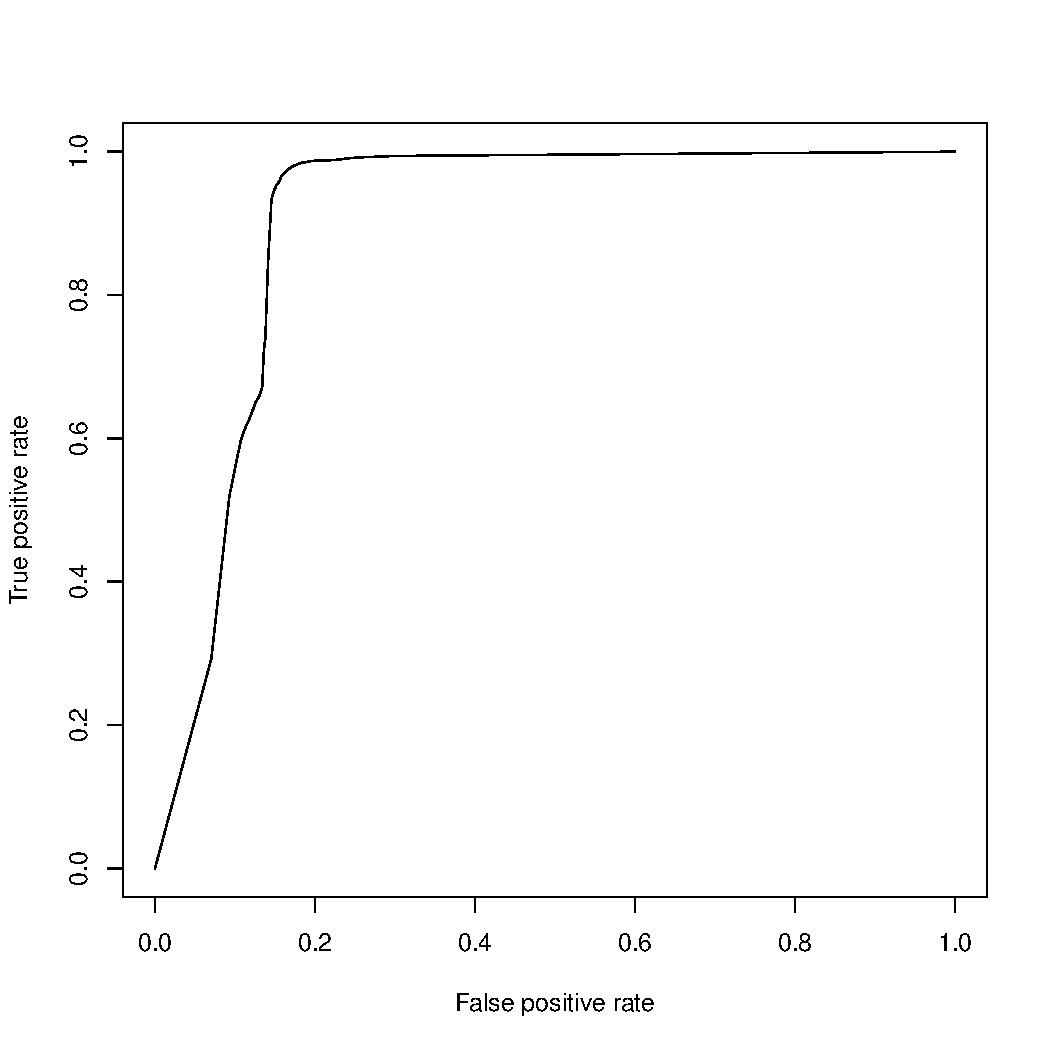
\includegraphics[width=\linewidth]{ROC_image4.pdf}
  \caption{Trained on image2}\label{}
\endminipage\hfill
\minipage{0.32\textwidth}%
  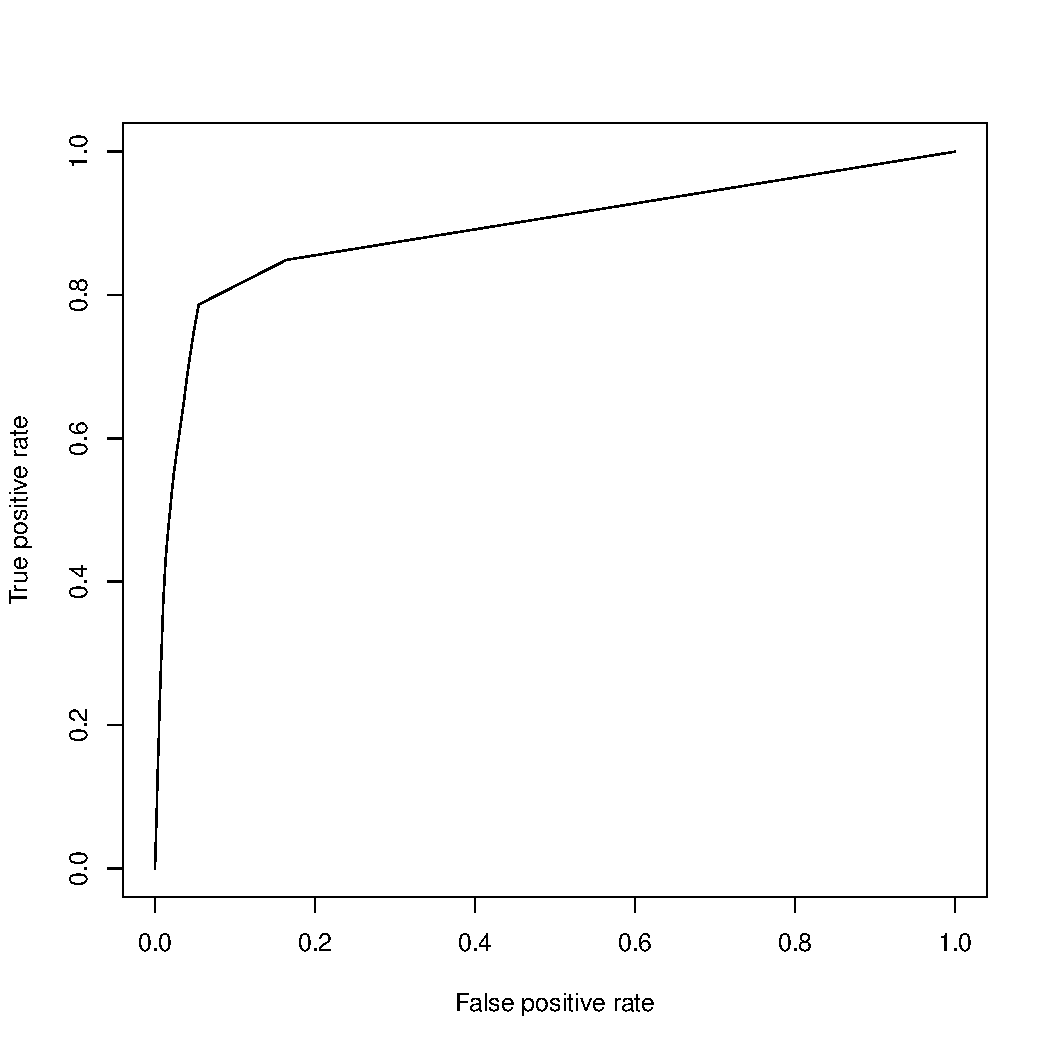
\includegraphics[width=\linewidth]{ROC_image8.pdf}
  \caption{Trained on image3}\label{}
\endminipage
\end{figure}


\section{Reproducibility}

{\bf How we organized out code and github repo}


 \begin{thebibliography}{1}

\bibitem{notes} Ben-Hur, A., Elisseeff, A., Guyon, I.: A stability based method for discovering structure in clustered data. In: Pacific Symposium on Biocomputing, pp. 6�17.   
\end{thebibliography}


\end{document}